\section{The M.I. Agent}\label{section:agent}
The purpose of the Agent is to translate the players actual position into a position on the screen.
It will do this, by estimating the players position, based on prior knowledge, constraints and sensor input.

\subsection{Agent constraints}
The agent will observe the environment and take actions based on a set of constraints and conditions.
All the agent's constraints is shown in \figref{figure:constraints} and will explained below.
\begin{enumerate}[label=(\alph*)]
\item Jitter noise is caused by tiny vibrations and occurs when the player is handling the device.
Therefore, the agent will ignore all acceleration-values between -0.1 and 0.1.
\item To simplify the complexity of the application, the movement-area will be a fixed size of 3 meters.
\item To help the agent decide whether a step is actually a step, a single step is limited to maximum of 100 cm.
\item A step must be at least 20 cm.
\item To ensure consistency in accelerometer readings, a player must hold the device as shown.
\item The velocity is limited to 3 m/s as the player should not be able to move faster than this.
\item %The accelerometer readings of the intended device cannot exceed gravitational pull more than 2g in positive/negative.
From observations, accelerations with a value exceeding 9.80 m/s

\end{enumerate}

\fxnote{Lav en tegning. http://upload.wikimedia.org/wikipedia/commons/9/91/Simple_reflex_agent.png}



\begin{figure}[H]
	\centering
	\begin{subfigure}[b]{0.9\textwidth}
		\centering
		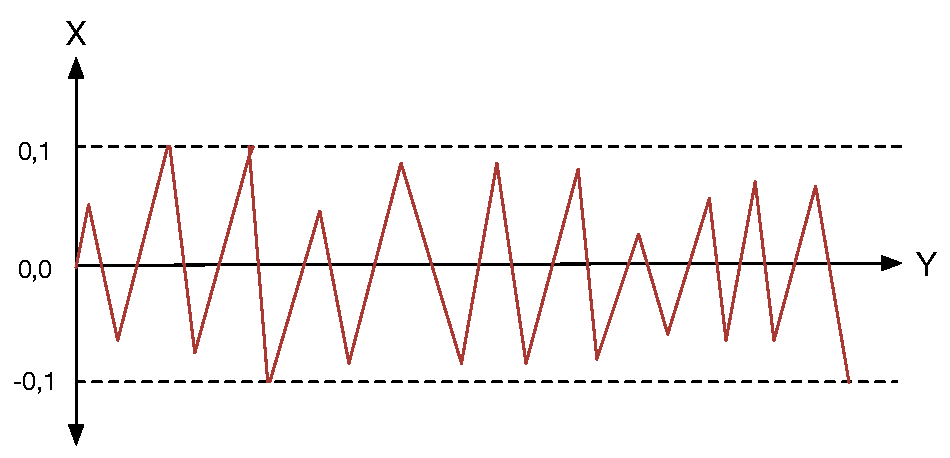
\includegraphics[scale = 0.45]{media/constraints/01-jitter-noise}
		\caption{Constraint 1: Jitter noise removal}
		\label{figure:jitter-noise}
	\end{subfigure}
	%---- linebreak	
	\begin{subfigure}[b]{0.45\textwidth}
		\centering
		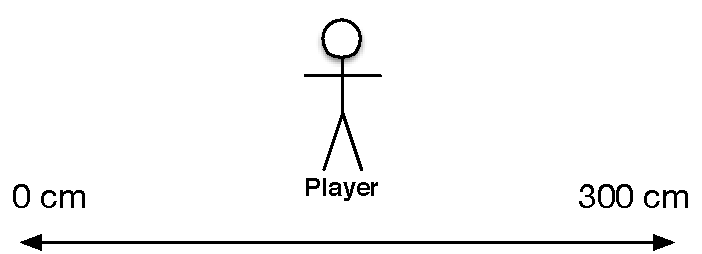
\includegraphics[scale = 0.45]{media/constraints/02-fixed-movement-area}
		\caption{Constraint 2: Fixed movement area}
		\label{figure:fixed-movement-area}
	\end{subfigure}
	\qquad
	\begin{subfigure}[b]{0.45\textwidth}
		\centering
		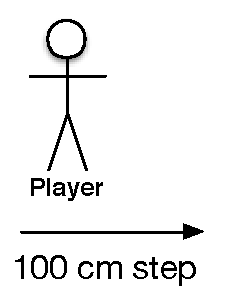
\includegraphics[scale = 0.45]{media/constraints/03-maximum-step}
		\caption{Constraint 3: Maximum step length}
		\label{figure:maximum-step}
	\end{subfigure}
	%---- linebreak
	\begin{subfigure}[b]{0.45\textwidth}
		\centering
		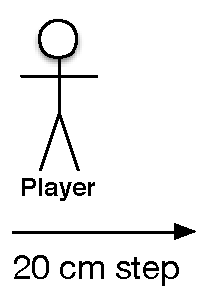
\includegraphics[scale = 0.45]{media/constraints/04-minimum-step}
		\caption{Constraint 4: Minimum step length}
		\label{figure:minimum-step}
	\end{subfigure}
	\qquad
	\begin{subfigure}[b]{0.45\textwidth}
		\centering
		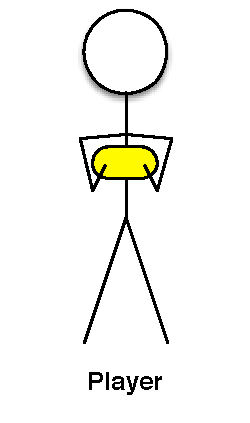
\includegraphics[scale = 0.45]{media/constraints/05-fixed-device-position}
		\caption{Constraint 5: Fixed device position}
		\label{figure:fixed-device-position}
	\end{subfigure}
	%---- linebreak
	\begin{subfigure}[b]{0.45\textwidth}
		\centering
		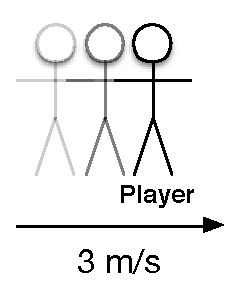
\includegraphics[scale = 0.45]{media/constraints/06-maximum-velocity}
		\caption{Constraint 6: Maximum velocity}
		\label{figure:maximum-velocity}
	\end{subfigure}
	\qquad
	\begin{subfigure}[b]{0.45\textwidth}
		\centering
		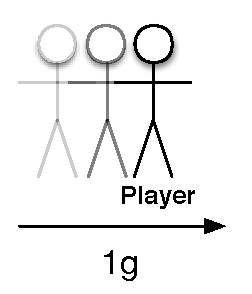
\includegraphics[scale = 0.45]{media/constraints/07-maximum-acceleration}
		\caption{Constraint 7: Maximum acceleration}
		\label{figure:maximum-acceleration}
	\end{subfigure}		
	\caption{}
	\label{figure:constraints}
\end{figure}




The agent will receive input from a device controlled by the player.
The input is the acceleration of the device's y-axis.
A velocity is then calculated by adding the acceleration to the existing velocity.

\subsection{Bayesian network}
The dynamic bayesian network (See \figref{fig:network}) shows how the different variables affect each other.
The current position ($pos_i$) is dependent on both the previously known position ($pos_{i-1}$) and the current velocity ($velo_i$).
The current velocity ($velo_i$) is dependent on the previously known velocity ($velo_{i-1}$) and the current acceleration ($acc_i$).
Using the constraints, the agent will estimate the probability of changing the players position on screen.


\begin{figure}[H]
\centering
\includegraphics[scale=0.7]{media/network}
\caption{}
\label{fig:network}
\end{figure}
